% $Author: oscar $
% $Date: 2009-09-15 16:53:48 +0200 (Tue, 15 Sep 2009) $
% $Revision: 29111 $
%=================================================================
\ifx\wholebook\relax\else
% --------------------------------------------
% Lulu:
	\documentclass[a4paper,10pt,twoside]{book}
	\usepackage[
		papersize={6.13in,9.21in},
		hmargin={.815in,.815in},
		vmargin={.98in,.98in},
		ignoreheadfoot
	]{geometry}
	\usepackage[hangul]{kotex}
	% $Author: oscar $
% $Date: 2009-09-13 20:58:29 +0200 (Sun, 13 Sep 2009) $
% $Revision: 29070 $
%=============================================================
% NB: documentclass must be set in main document.
% Allows book to be generated in multiple formats.
%=============================================================
%:Packages
\usepackage[T1]{fontenc}  %%%%%really important to get the code directly in the text!
\usepackage{palatino}
\usepackage{ifthen}
\usepackage{graphicx}
\graphicspath{{figures/}}
\usepackage{xspace}
\usepackage{makeidx}
\usepackage{isodateo} % enable \isodate
\usepackage{amssymb,textcomp}
%=============================================================
%:More packages
%\usepackage[english]{babel}
%\usepackage{lmodern}
%\usepackage[scaled=0.85]{helvet}
%\usepackage{microtype}
%\usepackage{theorem}
%\usepackage{float}
%\usepackage{longtable}
%\usepackage[nottoc]{tocbibind}
%\usepackage{multicol}
%\usepackage{booktabs}	% book-style tables
%\usepackage{topcapt}	% enables \topcaption
%\usepackage{multirow}
%\usepackage{tabularx}
%\usepackage{alltt}
\usepackage[usenames,dvipsnames]{color}
%\usepackage[hang]{subfigure}\makeatletter\def\p@subfigure{\thefigure\,}\makeatother
%\usepackage{rotating}
%\usepackage{enumitem}	% apb: allows more control over tags in enumerations
%\usepackage{verbatim}     % for comment environment
%\usepackage{varioref}	% for page references that work
%\usepackage{needspace}
%\usepackage[newparttoc]{titlesec}
%\usepackage{titletoc}
%\usepackage{wrapfig}
\usepackage[
	colorlinks=true,
	linkcolor=black,
	urlcolor=black,
	citecolor=black
]{hyperref}   % should come last
%=============================================================
%:URL style
\makeatletter
\def\url@leostyle{%
  \@ifundefined{selectfont}{\def\UrlFont{\sf}}{\def\UrlFont{\sffamily}}}
\makeatother
\urlstyle{leo}
%=============================================================
%:Booleans
\newboolean{lulu}
\setboolean{lulu}{false}
\newcommand{\ifluluelse}[2]{\ifthenelse{\boolean{lulu}}{#1}{#2}}
%=============================================================
%:Editorial comment macros
\newcommand{\nnbb}[2]{
  \fbox{\bfseries\sffamily\scriptsize#1}
  {\sf\small$\blacktriangleright$\textit{#2}$\blacktriangleleft$}
}
\newcommand{\on}[1]{\nnbb{Oscar}{#1}}
\newcommand{\here}{\nnbb{CONTINUE}{HERE}}
%=============================================================
%:Abbreviation macros
\newcommand{\ie}{\emph{i.e.},\xspace}
\newcommand{\eg}{\emph{e.g.},\xspace}
\newcommand{\etc}{\emph{etc.}\xspace}
\newcommand{\etal}{\emph{et al.}\xspace}
\newcommand{\straightquote}{"}
\newcommand{\sba}{\url{SquareBracketAssociates.org}\xspace}
%=============================================================
%:Patterns
% \newcommand{\pattern}[2]{\newpage\section{{\sf #1}}\label{pat:#2}}
% \newcommand{\pattern}[2]{\newpage\index{#1 (Pattern)}\section{#1}\label{pat:#2}}
\newcommand{\pattern}[2]{\cleardoublepage\index{#1 (패턴)}\section{#1}\label{pat:#2}}
\newcommand{\thumbnail}[2]{\index{#1 (패턴)}\subsection{#1}\label{pat:#2}}
\newcommand{\thumblang}[2]{\index{#1 (패턴 랭귀지)}\subsection{#1}\label{pat:#2}}
\newcommand{\variant}[1]{{\emph{#1}}\xspace}
% \newcommand{\problem}[1]{\subsection*{Problem}\emph{#1}}
\newcommand{\intent}[1]{\paragraph{의도}\emph{#1}}
\newcommand{\problem}[1]{\paragraph{문제}\emph{#1}}
\newcommand{\solution}[1]{\paragraph{해결}\emph{#1}}
\newcommand{\discussion}[0]{\paragraph{토론}}
\newcommand{\cmd}[1]{{\tt #1}\xspace}
%=============================================================
%:Environments
\newenvironment{bulletlist}{\begin{itemize}\setlength{\itemsep}{0ex}}
{\end{itemize}}
%=============================================================
%:Cross reference macros
\newcommand{\chalabel}[1]{\label{cha:#1}}
\newcommand{\seclabel}[1]{\label{sec:#1}}
\newcommand{\figlabel}[1]{\label{fig:#1}}
\newcommand{\tablabel}[1]{\label{tab:#1}}
\newcommand{\rulelabel}[1]{\label{rule:#1}}
\newcommand{\eglabel}[1]{\label{eg:#1}}
\newcommand{\scrlabel}[1]{\label{scr:#1}}
\newcommand{\mthlabel}[1]{\label{mth:#1}}
\newcommand{\clslabel}[1]{\label{cls:#1}}
\newcommand{\faqlabel}[1]{\label{faq:#1}}
%\newcommand{\charef}[1]{Chapter~\ref{cha:#1}\xspace}
%\newcommand{\secref}[1]{Section~\ref{sec:#1}\xspace}
\newcommand{\figref}[1]{Figure~\ref{fig:#1}\xspace}
% \newcommand{\patpgref}[2]{\hyperref[pat:#2]{\sf #1} [p.~\pageref{pat:#2}]\xspace}
\newcommand{\patpgref}[2]{\index{#1 (Pattern)}\hyperref[pat:#2]{#1} [p.~\pageref{pat:#2}]\xspace}
\newcommand{\patlangpgref}[2]{\index{#1 (Pattern language)}\hyperref[pat:#2]{#1} [p.~\pageref{pat:#2}]\xspace}
% \newcommand{\patref}[2]{\hyperref[pat:#2]{\sf #1}\xspace}
\newcommand{\patref}[2]{\index{#1 (Pattern)}\hyperref[pat:#2]{#1}\xspace}
\newcommand{\patlangref}[2]{\index{#1 (Pattern language)}\hyperref[pat:#2]{#1}\xspace}
% \newcommand{\charef}[2]{\hyperref[cha:#2]{\underline{\sf #1}}\xspace}
% \newcommand{\charef}[2]{\hyperref[cha:#2]{\sf #1}\xspace}
\newcommand{\charef}[2]{\index{#1 (Pattern cluster)}\hyperref[cha:#2]{#1}\xspace}
% \newcommand{\chapgref}[2]{\hyperref[cha:#2]{\sf #1} [p.~\pageref{cha:#2}]\xspace}
\newcommand{\chapgref}[2]{\index{#1 (Pattern cluster)}\hyperref[cha:#2]{#1} [p.~\pageref{cha:#2}]\xspace}
%\newcommand{\Figref}[1]{Figure~\ref{fig:#1}\xspace}
%\newcommand{\appref}[1]{Appendix~\ref{app:#1}\xspace}
%\newcommand{\tabref}[1]{Table~\ref{tab:#1}\xspace}
%\newcommand{\ruleref}[1]{\ref{rule:#1}\xspace}
%\newcommand{\egref}[1]{example~\ref{eg:#1}\xspace}
%\newcommand{\Egref}[1]{Example~\ref{eg:#1}\xspace}
%\newcommand{\scrref}[1]{script~\ref{scr:#1}\xspace}
%\newcommand{\Scrref}[1]{Script~\ref{scr:#1}\xspace}
%\newcommand{\tscrref}[1]{the script~\ref{scr:#1}\xspace}
%\newcommand{\Tscrref}[1]{The script~\ref{scr:#1}\xspace}
%\newcommand{\mthref}[1]{method~\ref{mth:#1}\xspace}
%\newcommand{\mthsref}[1]{methods~\ref{mth:#1}\xspace}
%\newcommand{\Mthref}[1]{Method~\ref{mth:#1}\xspace}
%\newcommand{\tmthref}[1]{the method~\ref{mth:#1}\xspace}
%\newcommand{\Tmthref}[1]{The method~\ref{mth:#1}\xspace}
%\newcommand{\clsref}[1]{class~\ref{cls:#1}\xspace}
%\newcommand{\tclsref}[1]{the class~\ref{cls:#1}\xspace}
%\newcommand{\Tclsref}[1]{The class~\ref{cls:#1}\xspace}
%=============================================================
%:Page Layout
\setlength{\headsep}{1cm}
%=============================================================
%:Menu item macro
%\definecolor{lightgray}{gray}{0.89}
%\newcommand{\menu}[1]{{%
%	\setlength{\fboxsep}{0pt}%
%	\colorbox{lightgray}{{{\upshape\sffamily\strut \,#1\,}}}}}
%\newcommand{\go}{\,$\triangleright$\,}
%\newcommand{\short}[1]{\mbox{{\sc cmd}\hspace{0.08em}--\hspace{0.09em}#1}\xspace}
%\newcommand{\button}[1]{{%
%	\setlength{\fboxsep}{0pt}%
%	\fbox{{\upshape\sffamily\strut \,#1\,}}}}
%\newcommand{\toolsflap}{\textit{Tools} flap\xspace}
%=============================================================
%:Section depth
%\setcounter{secnumdepth}{2}
%
%\DeclareGraphicsExtensions{.pdf, .jpg, .png}
%=============================================================
%:PDF setup
\hypersetup{
   pdftitle={Object-Oriented Reengineering Patterns},
   pdfauthor={Serge Demeyer, St\'ephane Ducasse, Oscar Nierstrasz},
   pdfkeywords={Reengineering, Object-Oriented Programming, Patterns},
   pdfsubject={Computer Science}
}
%=============================================================
%:Page layout and appearance
%\renewcommand{\chaptermark}[1]{\markboth{#1}{}}
%\renewcommand{\sectionmark}[1]{\markright{\thesection\ #1}}
%\renewpagestyle{plain}[\small\itshape]{%
%	\setheadrule{0pt}%
%	\sethead[][][]{}{}{}%
%	\setfoot[][][]{}{}{}}
%\renewpagestyle{headings}[\small\itshape]{%
%	\setheadrule{0pt}%
%	\setmarks{chapter}{section}%
%	\sethead[\thepage][][\chaptertitle]{\sectiontitle}{}{\thepage}%
%	\setfoot[][][]{}{}{}}
%=============================================================
%:Title section setup and TOC numbering depth
%\setcounter{secnumdepth}{1}
%\setcounter{tocdepth}{1}
%\titleformat{\part}[display]{\centering}{\huge\partname\ \thepart}{1em}{\Huge\textbf}[]
%\titleformat{\chapter}[display]{}{\huge\chaptertitlename\ \thechapter}{1em}{\Huge\raggedright\textbf}[]
%\titlecontents{part}[3pc]{%
%		\pagebreak[2]\addvspace{1em plus.4em minus.2em}%
%		\leavevmode\large\bfseries}
%	{\contentslabel{3pc}}{\hspace*{-3pc}}
%	{}[\nopagebreak]
%\titlecontents{chapter}[3pc]{%
%		\pagebreak[0]\addvspace{1em plus.2em minus.2em}%
%		\leavevmode\bfseries}
%	{\contentslabel{3pc}}{}
%	{\hfill\contentspage}[\nopagebreak]
%\dottedcontents{section}[3pc]{}{3pc}{1pc}
%\dottedcontents{subsection}[3pc]{}{0pc}{1pc}
%\let\origdoublepage\cleardoublepage
%\newcommand{\clearemptydoublepage}{%
%  \clearpage
%  {\pagestyle{empty}\origdoublepage}}
%\let\cleardoublepage\clearemptydoublepage % see http://www.tex.ac.uk/cgi-bin/texfaq2html?label=patch
%=============================================================
%:Listings package configuration
\newcommand{\caret}{\makebox{\raisebox{0.4ex}{\footnotesize{$\wedge$}}}}
% \newcommand{\escape}{{\sf \textbackslash}}
\definecolor{source}{gray}{0.95}
\usepackage{listings}
\lstdefinelanguage{Smalltalk}{
  morestring=[d]',
% Adapt this to other languages!
%  morecomment=[s]{"}{"},
  alsoletter={\#:},
  %escapechar={!},
  literate=
    {BANG}{!}1
%    {UNDERSCORE}{\_}1
    {\\st}{Smalltalk}9 % convenience -- in case \st occurs in code
    % {'}{{\textquotesingle}}1 % replaced by upquote=true in \lstset
%    {_}{{$\leftarrow$}}1
    {>>>}{{\sep}}1
    {^}{{$\uparrow$}}1
    {~}{{$\sim$}}1
    {-}{{\sf -\hspace{-0.13em}-}}1  % the goal is to make - the same width as +
    {+}{\raisebox{0.08ex}{+}}1		% and to raise + off the baseline to match -
    {-->}{{\quad$\longrightarrow$\quad}}3
	, % Don't forget the comma at the end!
  tabsize=4
}[keywords,comments,strings]

\lstset{language=Smalltalk,
	basicstyle=\sffamily,
	keywordstyle=\color{black}\bfseries,
	% stringstyle=\ttfamily, % Ugly! do we really want this? -- on
	mathescape=true,
	showstringspaces=false,
	keepspaces=true,
	breaklines=true,
	breakautoindent=true,
	backgroundcolor=\color{source},
	lineskip={-1pt}, % Ugly hack
	upquote=true, % straight quote; requires textcomp package
	columns=fullflexible} % no fixed width fonts
% \newcommand{\ct}{\lstinline[mathescape=false,basicstyle={\sffamily\upshape}]}
\newcommand{\ct}{\lstinline[mathescape=false,backgroundcolor=\color{white},basicstyle={\sffamily\upshape}]}
\newcommand{\lct}[1]{{\textsf{\textup{#1}}}}
%\newcommand{\scat}[1]{\emph{\textsf{#1}}\xspace}
%\newcommand{\prot}[1]{\emph{\textsf{#1}}\xspace}
% NB: No argument!
\lstnewenvironment{code}[0]{%
	\lstset{%
		% frame=lines,
		frame=single,
		framerule=0pt,
		mathescape=false
	}
}{}
%\def\ignoredollar#1{}
%=============================================================
%:Reserving space
%\newcommand{\needlines}[1]{\Needspace{#1\baselineskip}}
%=============================================================
%:Indexing macros
% Macros ending with "ind" generate text as well as an index entry
% Macros ending with "index" *only* generate an index entry
\newcommand{\ind}[1]{\index{#1}#1\xspace} % plain text
\newcommand{\subind}[2]{\index{#1!#2}#2\xspace} % show #2, subindex under #1
\newcommand{\emphind}[1]{\index{#1}\emph{#1}\xspace} % emph #1
\newcommand{\emphsubind}[2]{\index{#1!#2}\emph{#2}\xspace} % show emph #2, subindex under #1
\newcommand{\patind}[1]{\index{#1@#1 (pattern)}\ct{#1}\xspace} % pattern
\newcommand{\seeindex}[2]{\index{#1|see{#2}}} % #1, see #2
%\newcommand{\boldidx}[1]{{\bf #1}} % breaks hyperlink
%\newcommand{\indmain}[1]{\index{#1}#1\xspace} 
%\newcommand{\emphsubindmain}[2]{\index{#1!#2}\emph{#2}\xspace} % subindex, main entry
%\newcommand{\subindmain}[2]{\index{#1!#2}#2\xspace} % subindex, main entry
%\newcommand{\clsindmain}[1]{\index{#1!\#@(class)}\ct{#1}\xspace} % class main
%\newcommand{\indexmain}[1]{\index{#1}} 
%=============================================================
\parskip 1ex
%=============================================================

	\pagestyle{headings}
	\setboolean{lulu}{true}
% --------------------------------------------
% A4:
%	\documentclass[a4paper,11pt,twoside]{book}
%	% $Author: oscar $
% $Date: 2009-09-13 20:58:29 +0200 (Sun, 13 Sep 2009) $
% $Revision: 29070 $
%=============================================================
% NB: documentclass must be set in main document.
% Allows book to be generated in multiple formats.
%=============================================================
%:Packages
\usepackage[T1]{fontenc}  %%%%%really important to get the code directly in the text!
\usepackage{palatino}
\usepackage{ifthen}
\usepackage{graphicx}
\graphicspath{{figures/}}
\usepackage{xspace}
\usepackage{makeidx}
\usepackage{isodateo} % enable \isodate
\usepackage{amssymb,textcomp}
%=============================================================
%:More packages
%\usepackage[english]{babel}
%\usepackage{lmodern}
%\usepackage[scaled=0.85]{helvet}
%\usepackage{microtype}
%\usepackage{theorem}
%\usepackage{float}
%\usepackage{longtable}
%\usepackage[nottoc]{tocbibind}
%\usepackage{multicol}
%\usepackage{booktabs}	% book-style tables
%\usepackage{topcapt}	% enables \topcaption
%\usepackage{multirow}
%\usepackage{tabularx}
%\usepackage{alltt}
\usepackage[usenames,dvipsnames]{color}
%\usepackage[hang]{subfigure}\makeatletter\def\p@subfigure{\thefigure\,}\makeatother
%\usepackage{rotating}
%\usepackage{enumitem}	% apb: allows more control over tags in enumerations
%\usepackage{verbatim}     % for comment environment
%\usepackage{varioref}	% for page references that work
%\usepackage{needspace}
%\usepackage[newparttoc]{titlesec}
%\usepackage{titletoc}
%\usepackage{wrapfig}
\usepackage[
	colorlinks=true,
	linkcolor=black,
	urlcolor=black,
	citecolor=black
]{hyperref}   % should come last
%=============================================================
%:URL style
\makeatletter
\def\url@leostyle{%
  \@ifundefined{selectfont}{\def\UrlFont{\sf}}{\def\UrlFont{\sffamily}}}
\makeatother
\urlstyle{leo}
%=============================================================
%:Booleans
\newboolean{lulu}
\setboolean{lulu}{false}
\newcommand{\ifluluelse}[2]{\ifthenelse{\boolean{lulu}}{#1}{#2}}
%=============================================================
%:Editorial comment macros
\newcommand{\nnbb}[2]{
  \fbox{\bfseries\sffamily\scriptsize#1}
  {\sf\small$\blacktriangleright$\textit{#2}$\blacktriangleleft$}
}
\newcommand{\on}[1]{\nnbb{Oscar}{#1}}
\newcommand{\here}{\nnbb{CONTINUE}{HERE}}
%=============================================================
%:Abbreviation macros
\newcommand{\ie}{\emph{i.e.},\xspace}
\newcommand{\eg}{\emph{e.g.},\xspace}
\newcommand{\etc}{\emph{etc.}\xspace}
\newcommand{\etal}{\emph{et al.}\xspace}
\newcommand{\straightquote}{"}
\newcommand{\sba}{\url{SquareBracketAssociates.org}\xspace}
%=============================================================
%:Patterns
% \newcommand{\pattern}[2]{\newpage\section{{\sf #1}}\label{pat:#2}}
% \newcommand{\pattern}[2]{\newpage\index{#1 (Pattern)}\section{#1}\label{pat:#2}}
\newcommand{\pattern}[2]{\cleardoublepage\index{#1 (패턴)}\section{#1}\label{pat:#2}}
\newcommand{\thumbnail}[2]{\index{#1 (패턴)}\subsection{#1}\label{pat:#2}}
\newcommand{\thumblang}[2]{\index{#1 (패턴 랭귀지)}\subsection{#1}\label{pat:#2}}
\newcommand{\variant}[1]{{\emph{#1}}\xspace}
% \newcommand{\problem}[1]{\subsection*{Problem}\emph{#1}}
\newcommand{\intent}[1]{\paragraph{의도}\emph{#1}}
\newcommand{\problem}[1]{\paragraph{문제}\emph{#1}}
\newcommand{\solution}[1]{\paragraph{해결}\emph{#1}}
\newcommand{\discussion}[0]{\paragraph{토론}}
\newcommand{\cmd}[1]{{\tt #1}\xspace}
%=============================================================
%:Environments
\newenvironment{bulletlist}{\begin{itemize}\setlength{\itemsep}{0ex}}
{\end{itemize}}
%=============================================================
%:Cross reference macros
\newcommand{\chalabel}[1]{\label{cha:#1}}
\newcommand{\seclabel}[1]{\label{sec:#1}}
\newcommand{\figlabel}[1]{\label{fig:#1}}
\newcommand{\tablabel}[1]{\label{tab:#1}}
\newcommand{\rulelabel}[1]{\label{rule:#1}}
\newcommand{\eglabel}[1]{\label{eg:#1}}
\newcommand{\scrlabel}[1]{\label{scr:#1}}
\newcommand{\mthlabel}[1]{\label{mth:#1}}
\newcommand{\clslabel}[1]{\label{cls:#1}}
\newcommand{\faqlabel}[1]{\label{faq:#1}}
%\newcommand{\charef}[1]{Chapter~\ref{cha:#1}\xspace}
%\newcommand{\secref}[1]{Section~\ref{sec:#1}\xspace}
\newcommand{\figref}[1]{Figure~\ref{fig:#1}\xspace}
% \newcommand{\patpgref}[2]{\hyperref[pat:#2]{\sf #1} [p.~\pageref{pat:#2}]\xspace}
\newcommand{\patpgref}[2]{\index{#1 (Pattern)}\hyperref[pat:#2]{#1} [p.~\pageref{pat:#2}]\xspace}
\newcommand{\patlangpgref}[2]{\index{#1 (Pattern language)}\hyperref[pat:#2]{#1} [p.~\pageref{pat:#2}]\xspace}
% \newcommand{\patref}[2]{\hyperref[pat:#2]{\sf #1}\xspace}
\newcommand{\patref}[2]{\index{#1 (Pattern)}\hyperref[pat:#2]{#1}\xspace}
\newcommand{\patlangref}[2]{\index{#1 (Pattern language)}\hyperref[pat:#2]{#1}\xspace}
% \newcommand{\charef}[2]{\hyperref[cha:#2]{\underline{\sf #1}}\xspace}
% \newcommand{\charef}[2]{\hyperref[cha:#2]{\sf #1}\xspace}
\newcommand{\charef}[2]{\index{#1 (Pattern cluster)}\hyperref[cha:#2]{#1}\xspace}
% \newcommand{\chapgref}[2]{\hyperref[cha:#2]{\sf #1} [p.~\pageref{cha:#2}]\xspace}
\newcommand{\chapgref}[2]{\index{#1 (Pattern cluster)}\hyperref[cha:#2]{#1} [p.~\pageref{cha:#2}]\xspace}
%\newcommand{\Figref}[1]{Figure~\ref{fig:#1}\xspace}
%\newcommand{\appref}[1]{Appendix~\ref{app:#1}\xspace}
%\newcommand{\tabref}[1]{Table~\ref{tab:#1}\xspace}
%\newcommand{\ruleref}[1]{\ref{rule:#1}\xspace}
%\newcommand{\egref}[1]{example~\ref{eg:#1}\xspace}
%\newcommand{\Egref}[1]{Example~\ref{eg:#1}\xspace}
%\newcommand{\scrref}[1]{script~\ref{scr:#1}\xspace}
%\newcommand{\Scrref}[1]{Script~\ref{scr:#1}\xspace}
%\newcommand{\tscrref}[1]{the script~\ref{scr:#1}\xspace}
%\newcommand{\Tscrref}[1]{The script~\ref{scr:#1}\xspace}
%\newcommand{\mthref}[1]{method~\ref{mth:#1}\xspace}
%\newcommand{\mthsref}[1]{methods~\ref{mth:#1}\xspace}
%\newcommand{\Mthref}[1]{Method~\ref{mth:#1}\xspace}
%\newcommand{\tmthref}[1]{the method~\ref{mth:#1}\xspace}
%\newcommand{\Tmthref}[1]{The method~\ref{mth:#1}\xspace}
%\newcommand{\clsref}[1]{class~\ref{cls:#1}\xspace}
%\newcommand{\tclsref}[1]{the class~\ref{cls:#1}\xspace}
%\newcommand{\Tclsref}[1]{The class~\ref{cls:#1}\xspace}
%=============================================================
%:Page Layout
\setlength{\headsep}{1cm}
%=============================================================
%:Menu item macro
%\definecolor{lightgray}{gray}{0.89}
%\newcommand{\menu}[1]{{%
%	\setlength{\fboxsep}{0pt}%
%	\colorbox{lightgray}{{{\upshape\sffamily\strut \,#1\,}}}}}
%\newcommand{\go}{\,$\triangleright$\,}
%\newcommand{\short}[1]{\mbox{{\sc cmd}\hspace{0.08em}--\hspace{0.09em}#1}\xspace}
%\newcommand{\button}[1]{{%
%	\setlength{\fboxsep}{0pt}%
%	\fbox{{\upshape\sffamily\strut \,#1\,}}}}
%\newcommand{\toolsflap}{\textit{Tools} flap\xspace}
%=============================================================
%:Section depth
%\setcounter{secnumdepth}{2}
%
%\DeclareGraphicsExtensions{.pdf, .jpg, .png}
%=============================================================
%:PDF setup
\hypersetup{
   pdftitle={Object-Oriented Reengineering Patterns},
   pdfauthor={Serge Demeyer, St\'ephane Ducasse, Oscar Nierstrasz},
   pdfkeywords={Reengineering, Object-Oriented Programming, Patterns},
   pdfsubject={Computer Science}
}
%=============================================================
%:Page layout and appearance
%\renewcommand{\chaptermark}[1]{\markboth{#1}{}}
%\renewcommand{\sectionmark}[1]{\markright{\thesection\ #1}}
%\renewpagestyle{plain}[\small\itshape]{%
%	\setheadrule{0pt}%
%	\sethead[][][]{}{}{}%
%	\setfoot[][][]{}{}{}}
%\renewpagestyle{headings}[\small\itshape]{%
%	\setheadrule{0pt}%
%	\setmarks{chapter}{section}%
%	\sethead[\thepage][][\chaptertitle]{\sectiontitle}{}{\thepage}%
%	\setfoot[][][]{}{}{}}
%=============================================================
%:Title section setup and TOC numbering depth
%\setcounter{secnumdepth}{1}
%\setcounter{tocdepth}{1}
%\titleformat{\part}[display]{\centering}{\huge\partname\ \thepart}{1em}{\Huge\textbf}[]
%\titleformat{\chapter}[display]{}{\huge\chaptertitlename\ \thechapter}{1em}{\Huge\raggedright\textbf}[]
%\titlecontents{part}[3pc]{%
%		\pagebreak[2]\addvspace{1em plus.4em minus.2em}%
%		\leavevmode\large\bfseries}
%	{\contentslabel{3pc}}{\hspace*{-3pc}}
%	{}[\nopagebreak]
%\titlecontents{chapter}[3pc]{%
%		\pagebreak[0]\addvspace{1em plus.2em minus.2em}%
%		\leavevmode\bfseries}
%	{\contentslabel{3pc}}{}
%	{\hfill\contentspage}[\nopagebreak]
%\dottedcontents{section}[3pc]{}{3pc}{1pc}
%\dottedcontents{subsection}[3pc]{}{0pc}{1pc}
%\let\origdoublepage\cleardoublepage
%\newcommand{\clearemptydoublepage}{%
%  \clearpage
%  {\pagestyle{empty}\origdoublepage}}
%\let\cleardoublepage\clearemptydoublepage % see http://www.tex.ac.uk/cgi-bin/texfaq2html?label=patch
%=============================================================
%:Listings package configuration
\newcommand{\caret}{\makebox{\raisebox{0.4ex}{\footnotesize{$\wedge$}}}}
% \newcommand{\escape}{{\sf \textbackslash}}
\definecolor{source}{gray}{0.95}
\usepackage{listings}
\lstdefinelanguage{Smalltalk}{
  morestring=[d]',
% Adapt this to other languages!
%  morecomment=[s]{"}{"},
  alsoletter={\#:},
  %escapechar={!},
  literate=
    {BANG}{!}1
%    {UNDERSCORE}{\_}1
    {\\st}{Smalltalk}9 % convenience -- in case \st occurs in code
    % {'}{{\textquotesingle}}1 % replaced by upquote=true in \lstset
%    {_}{{$\leftarrow$}}1
    {>>>}{{\sep}}1
    {^}{{$\uparrow$}}1
    {~}{{$\sim$}}1
    {-}{{\sf -\hspace{-0.13em}-}}1  % the goal is to make - the same width as +
    {+}{\raisebox{0.08ex}{+}}1		% and to raise + off the baseline to match -
    {-->}{{\quad$\longrightarrow$\quad}}3
	, % Don't forget the comma at the end!
  tabsize=4
}[keywords,comments,strings]

\lstset{language=Smalltalk,
	basicstyle=\sffamily,
	keywordstyle=\color{black}\bfseries,
	% stringstyle=\ttfamily, % Ugly! do we really want this? -- on
	mathescape=true,
	showstringspaces=false,
	keepspaces=true,
	breaklines=true,
	breakautoindent=true,
	backgroundcolor=\color{source},
	lineskip={-1pt}, % Ugly hack
	upquote=true, % straight quote; requires textcomp package
	columns=fullflexible} % no fixed width fonts
% \newcommand{\ct}{\lstinline[mathescape=false,basicstyle={\sffamily\upshape}]}
\newcommand{\ct}{\lstinline[mathescape=false,backgroundcolor=\color{white},basicstyle={\sffamily\upshape}]}
\newcommand{\lct}[1]{{\textsf{\textup{#1}}}}
%\newcommand{\scat}[1]{\emph{\textsf{#1}}\xspace}
%\newcommand{\prot}[1]{\emph{\textsf{#1}}\xspace}
% NB: No argument!
\lstnewenvironment{code}[0]{%
	\lstset{%
		% frame=lines,
		frame=single,
		framerule=0pt,
		mathescape=false
	}
}{}
%\def\ignoredollar#1{}
%=============================================================
%:Reserving space
%\newcommand{\needlines}[1]{\Needspace{#1\baselineskip}}
%=============================================================
%:Indexing macros
% Macros ending with "ind" generate text as well as an index entry
% Macros ending with "index" *only* generate an index entry
\newcommand{\ind}[1]{\index{#1}#1\xspace} % plain text
\newcommand{\subind}[2]{\index{#1!#2}#2\xspace} % show #2, subindex under #1
\newcommand{\emphind}[1]{\index{#1}\emph{#1}\xspace} % emph #1
\newcommand{\emphsubind}[2]{\index{#1!#2}\emph{#2}\xspace} % show emph #2, subindex under #1
\newcommand{\patind}[1]{\index{#1@#1 (pattern)}\ct{#1}\xspace} % pattern
\newcommand{\seeindex}[2]{\index{#1|see{#2}}} % #1, see #2
%\newcommand{\boldidx}[1]{{\bf #1}} % breaks hyperlink
%\newcommand{\indmain}[1]{\index{#1}#1\xspace} 
%\newcommand{\emphsubindmain}[2]{\index{#1!#2}\emph{#2}\xspace} % subindex, main entry
%\newcommand{\subindmain}[2]{\index{#1!#2}#2\xspace} % subindex, main entry
%\newcommand{\clsindmain}[1]{\index{#1!\#@(class)}\ct{#1}\xspace} % class main
%\newcommand{\indexmain}[1]{\index{#1}} 
%=============================================================
\parskip 1ex
%=============================================================

%	\usepackage{a4wide}
% --------------------------------------------
	\begin{document}
	\renewcommand{\nnbb}[2]{} % Disable editorial comments
	\sloppy
\fi
%=================================================================
\chapter{중복 코드 감지}
\chalabel{DetectingDuplicatedCode}

\index{파울러, 마틴}
\index{벡, 켄트}
파울러와 벡은 소프트웨어 리팩터링의 필요성을 나타내는 상위 10가지 코드 스멜 중 첫 번째로 중복 코드(duplicated code)를 꼽았다 \cite{Fowl99a}. 그들이 설명하길, 코드를 복제할 때마다 나중에 비용을 지불해야 할 무언가(거의 기성품에 가까운 소프트웨어)를 지금 받는다는 의미에서 대출을 받는 것과 같다고 한다. 대출을 받는 것이 잘못된 것은 아니지만, 중복을 제거하기 위해 코드를 리팩터링하는 시간을 들여 지금 소액을 갚거나 (복잡성 및 유지 관리 비용의 증가로) 나중에 많은 금액을 갚는 것 중 하나를 선택할 수 있다.

경험적 연구 데이터에 따르면 일반적으로 산업용 소프트웨어의 8\%에서 12\%는 중복된 코드로 구성되어 있다 \cite{Duca99b}. 이 수치는 많지 않아 보일 수 있지만 실제로는 매우 높은 중복률을 달성하기 어렵습니다. (중복률이 50\%라도 되려면 얼마나 많은 노력이 필요할지 상상해 보자!) 따라서 15~20\%의 중복률은 심각한 것으로 간주된다. 

다음과 같은 이유로 중복 코드를 식별하는 것이 중요하다.

\begin{bulletlist}
\item 중복 코드는 구현된 모든 기능의 변형을 변경해야 하므로 변경 사항을 도입하는 데 방해가 된다. 일부 변형을 놓치기 쉬우므로 다른 곳에서 버그가 발생할 가능성이 높다.

\item 중복 코드는 시스템의 로직을 식별 가능한 산출물(클래스, 메서드, 패키지)로 그룹화하는 대신 복제하고 분산시킨다. 따라서 시스템을 이해하고 변경하기가 더 어려워진다. 논리적 부분 간의 관계를 이해하는 대신 먼저 식별한 다음 그 관계를 이해해야 한다.
\end{bulletlist}

중복 코드는 다양한 이유로 발생한다.

\begin{bulletlist}
\item 프로그래머가 이전에 수행한 작업과 원격으로 유사한 기능을 구현할 때마다 기존 코드를 새 작업의 모델로 사용하는 것은 당연하다. 기존 프로시저를 재조합하는 문제라면 작업은 간단할 것이다. 그러나 동작이 더 복잡한 경우 가장 쉬운 방법은 이전 코드를 복사, 붙여넣기 및 수정하여 기능을 달성하는 것이다. 이전 코드와 새 코드가 모두 다른 애플리케이션에 속한 경우 피해는 최소화된다. 하지만 같은 시스템에 속해 있다면 중복 코드가 발생하게 된다.

\item 때때로 다른 애플리케이션 또는 동일한 애플리케이션의 다른 버전 간에 코드를 복사, 붙여넣기 및 수정하는 경우가 있다. 여러 버전을 동시에 유지보수해야 하거나 서로 다른 애플리케이션 또는 버전을 병합해야 하는 경우 코드 중복 문제가 즉시 발생한다.
\end{bulletlist}

리엔지니어링 관점에서 보면 일반적으로 사람들은 시스템에 중복 문제가 있는지 여부를 알 수 있다. 첫째, 개발팀이나 관리자가 알려줄 것이다. 둘째, 일반적으로 프로젝트에서 중복이 발생했다는 몇 가지 분명한 징후가 있다. 예를 들어, 두 명의 개발자가 기존 코드를 복사하여 붙여넣지 않고는 8개월 이내에 4백만 줄의 코드를 개발할 수 없다. 시스템을 분석하는 동안 우연히 중복된 코드를 발견할 수도 있다. 그러나 시스템에 중복된 코드가 있다는 것을 아는 것과 정확히 어떤 부분이 중복되었는지 아는 것에는 큰 차이가 있다. 

\begin{figure}[h]
\begin{center}
\includegraphics[width=0.8\textwidth]{DuplicationMap}
\caption{\charef{중복 코드 감지}{DetectingDuplicatedCode}를 지원하는 두 가지 패턴.}
\figlabel{DuplicationMap}
\end{center}
\end{figure}

\subsection*{개요}

\charef{중복 코드 감지}{DetectingDuplicatedCode}는 두 가지 패턴으로 구성된다. 중복 코드를 감지하는 방법을 설명하는 \patref{기계적으로 코드 비교하기}{CompareCodeMechanically}, 그리고 간단한 이차원적 시각화를 통해 중복 코드를 더 잘 이해할 수 있는 방법을 보여주는 \patref{도트 플롯으로 코드 시각화하기}{VisualizeCodeAsDotplots}로 구성되어 있다.

시스템에서 중복을 감지하고 이해한 후에는 다양한 전략을 결정할 수 있다. \patpgref{메시드 추출하기}{ExtractMethod}와 같은 다양한 리팩터링 패턴을 사용하면 중복을 제거하는 데 도움이 될 수 있다. 중복은 책임이 잘못 배치되었다는 신호일 수 있으며, 이 경우 \patpgref{데이터 가까이 동작 이동하기}{MoveBehaviorCloseToData}를 해야 할 수도 있다. 

복잡한 조건문도 중복의 한 형태이며, 여러 클라이언트가 대상 클래스에 속해야 하는 동작을 중복해야 함을 나타낼 수 있다. 패턴 클러스터 \charef{다형성 적용된 조건문 변환}{TransformConditionalsTo다형성}을 사용하면 이러한 문제를 해결하는 데 도움이 될 수 있다.

%=================================================================
%:PATTERN -- {Compare Code Mechanically}
\pattern{기계적으로 코드 비교하기}{CompareCodeMechanically}

\intent{모든 소스 코드 파일을 한 줄씩 비교하여 \ind{중복 코드}(duplicated code) 발견하기.}

\subsection*{문제}

애플리케이션 코드의 어느 부분이 중복되었는지 어떻게 발견하는가?

\emph{이 문제는 다음과 같은 이유로 어렵다.} 

\begin{bulletlist}
\item 코드가 중복되었다고 의심할 수 있지만 중복이 발생한 위치에 대한 증거가 없다. 예를 들어 두 명의 프로그래머가 일부 코드를 복제하지 않고는 1년 동안 4백만 줄의 코드를 개발할 수 없다는 것을 알고 있다.

\item 코드를 검색하는 것은 중복을 발견하는 효과적인 방법이 아니며, 우연히 중복된 코드를 발견할 수 있을 뿐이다.

\item 프로그래머는 코드를 복사하여 붙여넣었을 뿐만 아니라 변수를 수정하거나 프로그램의 모양을 변경했을 수도 있다.
\end{bulletlist}

\emph{그러나 이 문제를 해결할 수 있는 이유는 다음과 같다.}

\begin{bulletlist}
\item 대부분의 중복 코드는 기계적 절차를 통해 감지할 수 있다.
\end{bulletlist}

\subsection*{해결}

소프트웨어 소스 코드의 각 줄을 다른 모든 코드 줄과 텍스트로 비교한다.

\subsubsection*{단계}

\begin{bulletlist}
\item 주석, 탭, 공백을 제거하여 코드 줄을 정규화한다.

\item 흥미롭지 않은 코드 요소가 포함된 줄을 제거한다(예: 그냥 \lct{else} 또는 \lct{\}}).

\item 각 줄을 다른 모든 줄과 비교한다. 해싱으로 검색 복잡성을 줄인다.

\begin{bulletlist}
\item 전처리: 각 줄의 해시 값 계산한다.
\item 실제 비교: 동일한 해시 버킷의 모든 줄을 비교한다.
\end{bulletlist}
\end{bulletlist}

\subsubsection*{변형}

이 방법은 변수 이름 변경으로 인해 중복된 코드의 일부 인스턴스를 식별하지 못할 수 있다. 모든 변수 식별자를 삭제하거나 공통 기호에 매핑하면 특정 식별자의 세부 사항을 추상화하면서 유사한 코드 패턴을 감지할 수 있다. 그러나 이 변형은 일부 코드의 시맨틱 처리(syntactic processing)를 필요로 한다. 

\subsection*{트레이드오프}

\subsubsection*{장점}

\begin{bulletlist}
\item 이 접근 방식은 간단하며 적당한 리소스만 사용해도 좋은 결과를 제공한다.

\item 전체 구문 분석기(parser)가 아니라 어휘 분석기(lexical analyzer)만 구축하면 된다는 점에서 언어에 거의 독립적이다. 그렇기 때문에 원하는 정교함의 수준에 따라 간단한 perl 스크립트로도 충분할 수 있다.

\item 간단한 통계와 비율은 쉽게 계산할 수 있으며 리소스 할당이나 신규 인력 채용에 대한 논의에서 신뢰성을 높이거나 더 많은 힘을 얻는데 도움이 될 수 있다.
\end{bulletlist}

\subsubsection*{단점}

\begin{bulletlist}
\item 복사 후 많이 편집된 코드는 중복된 코드로 식별하기 어려울 수 있다.

\item 중복 코드가 많이 포함된 시스템은 많은 데이터를 생성하여 효과적으로 분석하기 어려울 수 있다
\end{bulletlist}

\subsection*{예시}

코드 중복이 의심되는 C++로 작성된 시스템의 경우를 생각해 보자. 하지만 직접 코드를 작성하지 않았기 때문에 실제 중복이 어디에서 발생하는지 알 수 없다. 중복 코드 조각이 어디에 있는지 어떻게 감지할 수 있을까? 가장 간단한 방법은 먼저 코드를 정규화하여 코드에서 모든 공백을 제거한 다음 각 코드 줄을 자체적으로 비교하는 작은 스크립트를 작성하는 것이다.

정규화하면 다음 코드가 변경된다.

\begin{code}
...
// assign same fastid as container
fastid = NULL;
const char* fidptr = getFastid();
if(fidptr != NULL) {
	int l = strlen(fidptr);
	fastid = new char[l+1];
	char *tmp = (char*) fastid;
	for (int i =0;i<l;i++)
		tmp[i] = fidptr[i];
	tmp[l] = '\0';
}
...
\end{code}
into
\begin{code}
...
fastid=NULL;
constchar*fidptr=getFastid();
if(fidptr!=NULL)
intl=strlen(fidptr);
fastid=newchar[l+1];
char*tmp=(char*)fastid;
for(inti=0;i<l;i++)
tmp[i]=fidptr[i];
tmp[l]='\0';
...
\end{code}

그 후 코드를 한 줄씩 비교하면 중복된 줄의 순서를 알려주는 보고서가 생성된다.

\begin{code}
Lines:fastid=NULL;;constchar*fidptr=getFastid();;if(fidptr!=NULL);
intl=strlen(fidptr);;fastid=newchar[l+1];;
Locations:
</typesystem/Parser.C>6178/6179/6180/6181/6182
</typesystem/Parser.C>6198/6199/6200/6201/6202
\end{code}

다음은 이 기능을 수행하는 perl 스크립트 샘플이다.

\begin{code}
#! /usr/bin/env perl -w
# duplocForCPP.pl - detect duplicated lines of code (algorithm only)
# Synopsis: duplocForCPP.pl filename ...
# Takes code (or other) files and collects all line numbers of lines
# equal to each other within these files. The algorithm is linear (in
# space and time) to the number of lines in input.

# Output: Lists of numbers of equal lines.
# Author: Matthias Rieger

$equivalenceClassMinimalSize = 1;
$slidingWindowSize  = 5;
$removeKeywords = 0;

@keywords = qw(if
		then
		else
		for
		{
		}
	);

$keywordsRegExp = join '|', @keywords;

@unwantedLines = qw( else
		return
		return;
		return result;
		}else{
		#else
		#endif
		{
		}
		;
		};
	);
push @unwantedLines, @keywords;

@unwantedLines{@unwantedLines} = (1) x @unwantedLines;

$totalLines = 0;
$emptyLines = 0;
$codeLines = 0;
@currentLines = ();
@currentLineNos = ();
%eqLines = ();
$inComment = 0;

$start = (times)[0];

while (<>) {
	chomp;
	$totalLines++;

	# remove comments of type /* */
	my $codeOnly = ";
	while(($inComment && m|\*/|) || (!$inComment && m|/\*|)) {
		unless($inComment) { $codeOnly .= $` }
		$inComment = !$inComment;
		$_ = $';
	}
	$codeOnly .= $_ unless $inComment;
	$_ = $codeOnly;

	s|//.*$||; # remove comments of type //
	s/\s+//g;  #remove white space
	s/$keywordsRegExp//og if $removeKeywords; #remove keywords

	# remove empty and unwanted lines
	if((!$_ && $emptyLines++)
		|| (defined $unwantedLines{$_} && $codeLines++)) { next }

	$codeLines++;
	push @currentLines, $_;
	push @currentLineNos, $.;
	if($slidingWindowSize < @currentLines) {
		shift @currentLines;
		shift @currentLineNos;
	}

	# print STDERR "Line $totalLines >$_<\n";

	my $lineToBeCompared = join ", @currentLines;
	my $lineNumbersCompared = "<$ARGV>"; # append the name of the file
	$lineNumbersCompared .= join '/', @currentLineNos;
	# print STDERR "$lineNumbersCompared\n";
	if($bucketRef = $eqLines{$lineToBeCompared}) {
		push @$bucketRef, $lineNumbersCompared;
	} else {
		$eqLines{$lineToBeCompared} = [ $lineNumbersCompared ];
	}

	if(eof) { close ARGV } # Reset linenumber-count for next file
}

$end = (times)[0];
$processingTime = $end - $start;

# print the equivalence classes

$numOfMarkedEquivClasses = 0;
$numOfMarkedElements = 0;
foreach $line (sort { length $a <=> length $b } keys %eqLines) {
	if(scalar @{$eqLines{$line}} > $equivalenceClassMinimalSize) {
		$numOfMarkedEquivClasses++;
		$numOfMarkedElements += scalar @{$eqLines{$line}};
		print "Lines: $line\n";
		print "Locations: @{$eqLines{$line}}\n\n";
	}
}

print "\n\n\n";
print "Number of Lines processed: $totalLines\n";
print "Number of Empty Lines: $emptyLines\n";
print "Number of Code Lines: $codeLines\n";
print "Scanning time in seconds: $processingTime\n";
print "Lines per second: @{[$totalLines/$processingTime]}\n";
print "--------------------------------------\n";
print "Total Number of equivalence classes: @{[scalar keys %eqLines]}\n";
print "Size of Sliding window: $slidingWindowSize\n";
print "Lower bound of eqiv-class Size: $equivalenceClassMinimalSize\n";
print "Number of marked equivalence classes: $numOfMarkedEquivClasses\n";
print "Number of marked elements: $numOfMarkedElements\n";
\end{code}

\subsection*{알려진 용도}

소프트웨어 리엔지니어링의 맥락에서, 이 패턴은 최대 100만 줄의 \ind{C++}가 포함된 FAMOOS 사례 연구에서 중복 코드를 탐지하는 데 적용되었다. 또한 4백만 줄의 코드가 포함된 \ind{COBOL} 시스템에서 중복 코드를 탐지하는 데도 적용되었다. \ind{DATRIX}는 대규모 통신 시스템의 여러 버전을 조사하여 총 8,900만 줄의 코드를 모두 \cite{Lagu97a}로 분석했다. 

%=================================================================
%:PATTERN -- {Visualize Code as Dotplots}
\pattern{도트 플롯으로 코드 시각화하기}{VisualizeCodeAsDotplots}


\intent{도트 플롯의 패턴을 연구하여 중복의 본질에 대한 통찰력을 얻는다.}

\subsection*{문제}

소프트웨어 시스템에서 코드 중복의 범위와 성격에 대한 통찰력을 어떻게 얻을 수 있는가?

\emph{이 문제는 다음과 같은 이유로 어렵다.} 

\begin{bulletlist}
\item 시스템에서 중복된 코드가 어디에 존재하는지 아는 것만으로는 그 성격을 이해하거나 이에 대해 무엇을 해야 하는지 파악하는 데 도움이 되지 않는다.
\end{bulletlist}

\emph{그러나 이 문제를 해결할 수 있는 이유는 다음과 같다.}

\begin{bulletlist}
\item 하나의 그림이 천 마디 말보다 가치가 있다.
\end{bulletlist}

\subsection*{해결}

두 축이 각각의 소스 코드 파일(동일한 파일일 수 있음)을 나타내는 행렬로 시각화하고 점들은 소스 코드 줄이 중복되는 곳에 표시한다.

\subsubsection*{단계}

두 개의 파일 A와 B를 분석하려는 경우 다음과 같다.

\begin{bulletlist}
\item 두 파일의 내용을 정규화하여 노이즈(공백 등)를 제거한다.

\item 행렬의 각 축이 정규화된 파일의 요소(예: 코드 줄)를 나타내도록 한다.

\item 두 요소 사이의 일치를 행렬에 점으로 표시한다.

\item 획득한 그림을 해석한다. 대각선은 두 파일 간에 중복된 코드를 나타낸다.
\end{bulletlist}

단일 파일 내부의 중복을 분석하기 위해 해당 파일의 요소를 양쪽 축에 플롯한다.

\subsubsection*{해석}

얻어진 행렬의 해석은 \figref{DuplicationDotplot}에 설명되어 있다.

\begin{figure}
\begin{center}
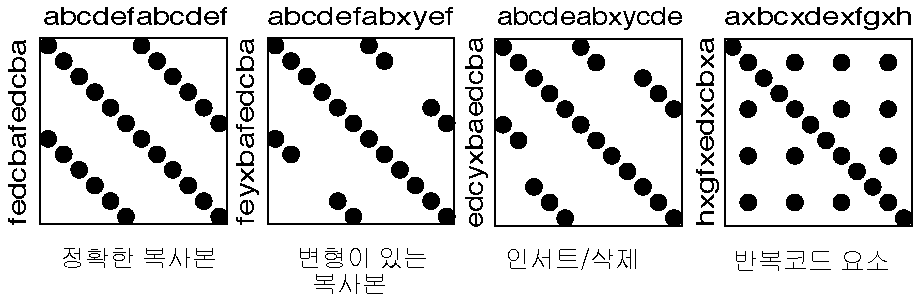
\includegraphics[width=\textwidth]{DuplicationDotplot}
\caption{가능한 점의 시퀀스 및 관련 해석.}
\figlabel{DuplicationDotplot}
\end{center}
\end{figure}

그림에 표시된 점으로 형성되는 몇 가지 흥미로운 구성은 다음과 같다.

\begin{bulletlist}
\item \emph{정확한 복사본:} 점의 대각선은 소스 코드의 복사된 시퀀스를 나타낸다.

\item \emph{변형이 있는 복사본:} 시퀀스에 구멍이 있는 것은 복사된 시퀀스의 일부가 변경되었음을 나타낸다.

\item \emph{인서트/삭제:} 오른쪽이나 왼쪽으로 이동된 부분이 있는 끊어진 시퀀스는 코드의 일부가 삽입되거나 삭제되었음을 나타낸다.

\item  \emph{반복코드 요소:} 직사각형 구성은 동일한 코드가 주기적으로 발생함을 나타낸다. 예를 들어 C 또는 C ++ 스위치 문의 개별 대소문자 끝의 쉼표나 \lct{\#ifdef 일부 조건}과 같은 반복되는 전처리기 명령이 있다.
\end{bulletlist}

\subsection*{트레이드오프}

\subsubsection*{장점}

\begin{bulletlist}
\item 이 접근 방식은 코드 정규화만 언어 구문에 의존하기 때문에 언어에 크게 구애받지 않는다.

\item 이 접근 방식은 도트 플롯을 통해 코드의 특정 부분을 더 자세히 살펴볼 수 있기 때문에 알려지지 않은 대량의 코드를 리버스 엔지니어링할 때 효과적이다.

\item 이 아이디어는 간단하지만 놀라울 정도로 잘 작동한다. 이 접근법의 간단한 버전은 유능한 프로그래머라면 적절한 도구를 사용하여 며칠 안에 구현할 수 있다. (실력 있는 학생 중 한 명은 이틀 만에 델파이로 작은 도트플롯 브라우저를 만들었다.)
\end{bulletlist}

\subsubsection*{단점}

\begin{bulletlist}
\item 도트 플롯은 쌍으로만 비교를 표시한다. 전체 소프트웨어 시스템에서 중복된 요소의 모든 인스턴스를 식별하는 데 반드시 도움이 되는 것은 아니다. 이 접근 방식을 쉽게 확장하여 각 축에 여러 파일을 표시할 수 있지만 여전히 비교는 쌍 단위로만 이루어진다.
\end{bulletlist}

\subsubsection*{어려움}

\begin{bulletlist}
\item 도트 플롯 시각화 도구의 나이브한 구현은 대규모 시스템의 확장이 쉽지 않을 수 있다. 대규모 데이터 집합에 맞게 접근 방식을 조정하고 최적화하면 접근 방식의 단순성이 저하될 수 있다.

\begin{figure}[t]
\begin{center}
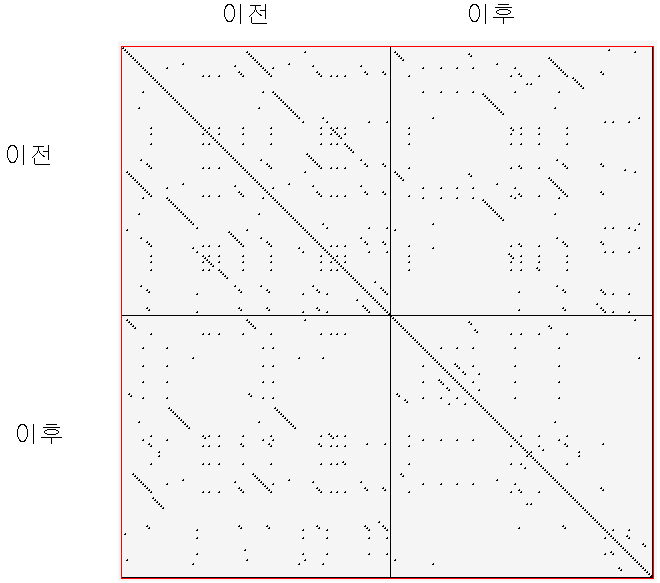
\includegraphics[width=0.8\textwidth]{DuplicationRefactoring}
\caption{리팩토링 전후의 코드 중복.}
\figlabel{DuplicationRefactoring}
\end{center}
\end{figure}

\item 데이터의 해석은 언뜻 보기보다 더 미묘할 수 있다. 실제로 여러 파일을 비교하는 동안 대각선은 실제보다 더 많은 중복을 나타내며, 이는 \figref{DuplicationRefactoring} 및 \figref{DuplicationPython}에 표시된 것처럼 여러 파일에서 중복된 조각을 비교하고 있기 때문이다.

\index{벽화 시각화}
\item 화면 크기는 시각화할 수 있는 정보의 양을 제한한다. 소위 ``벽화'' 시각화(mural visualization) 접근 방식인 \cite{Jerd96b}로 일부 성공을 거두었다. 그러나 이러한 기법은 단순한 도트 플롯보다 구현하기가 훨씬 더 어렵고 추가적인 노력을 기울일 가치는 없다.
\end{bulletlist}

\subsection*{예시}

\figref{DuplicationRefactoring}에서는 중복이 제거되기 전과 후의 두 가지 버전의 소프트웨어에 대한 \ind{dotplot}을 볼 수 있다. 첫 번째 버전은 왼쪽 위 사각형에 비교되어 있다. 대각선 아래 선은 모든 코드 줄이 그 자체와 비교되고 있음을 보여준다. 더 흥미로운 점은 도트 플롯에 여러 개의 다른 대각선이 나타나는데, 이는 이 파일 내에서 코드가 중복되었다는 것을 의미한다. 동일한 파일의 두 번째 버전이 오른쪽 아래 사각형에서 자신과 비교되고 있다. 여기에서는 주 대각선을 제외하고는 크게 중복된 부분이 없는데, 이는 중복된 코드가 모두 성공적으로 리팩터링되었다는 사실을 반영한다.

\begin{figure}[h]
\begin{center}
\includegraphics[width=\textwidth]{DuplicationPython}
\caption{파이썬 파일 A에 대해서 자신과 두 번째 파일 B를 비교하고 있다.}
\figlabel{DuplicationPython}
\end{center}
\end{figure}

왼쪽 아래 사각형과 오른쪽 위 사각형은 서로의 거울 이미지이다. 이전과 이후 파일이 어떻게 재구성되었는지 알려준다. 강한 대각선이 없으므로 상당한 재구성이 이루어졌음을 알 수 있다. 대각선 줄무늬는 이전 버전에서 어떤 부분이 살아남았고 새 버전에서 어디에 나타나는지 보여준다. 도트 플롯만 보면 코드의 약 절반이 살아남았고 나머지 절반의 코드가 크게 재작성되었음을 짐작할 수 있다.

도트 플롯은 여러 파일에서 중복을 감지하는 데도 유용하다. \figref{DuplicationPython}은 두 개의 \ind{Python} 파일을 비교한 도트 플롯을 보여준다. A와 A를 비교하면 본질적으로 내부 중복이 없음을 알 수 있다. 파일의 하단에는 매트릭스 패턴으로 표시된 스위치 문이 있을 가능성이 높다.

하지만 파일 A와 파일 B를 비교하면 엄청난 양의 중복을 발견할 수 있다. 파일 B는 파일 A를 다양한 방식으로 확장한 복사본에 불과한 것처럼 보인다. 자세히 조사한 결과 사실로 밝혀졌다. 실제로 파일 A는 실수로 릴리스에 남겨진 파일 B의 이전 버전에 불과했다.

도트 플롯은 다른 문제를 감지하는 데도 유용할 수 있다. \figref{DuplicationSwitch}는 개별 구성 코드를 호출하는 데 사용되는 유형 변수에 대한 스위치 문을 나타내는 네 개의 복제본을 표시한다. 중복된 코드는 아마도 \charef{다형성 적용한 조건문 변환}{TransformConditionalsToPolymorphism}을 적용하여 제거할 수 있을 것이다.

\begin{figure}
\begin{center}
\includegraphics[width=0.75\textwidth]{DuplicationSwitch}
\caption{4개의 스위치 문으로 생성된 도트 플롯이다.}
\figlabel{DuplicationSwitch}
\end{center}
\end{figure}

\subsection*{알려진 용도}

이 패턴은 생물학적 연구에 적용되어 DNA 서열 \cite{Pust82a}을 검출하는 데 사용되었다. 도트플롯 도구 \cite{Helf95a}는 수동 페이지, 문학 텍스트 및 파일 시스템의 이름에서 유사성을 감지하는 데 사용되었다. \ind{FAMOOS} 프로젝트에서 이 패턴은 소프트웨어 소스 코드의 중복을 식별하는 도구 \cite{Duca99b}인 \ind{Duploc}을 구축하는 데 적용되었다. \ind{Dup} 도구 \cite{Bake92a}는 X-Window 시스템의 소스 코드를 조사하는 데 사용되었으며, 도트 플롯 매트릭스 그래픽 표현을 사용한다.

\subsection*{관련 패턴}

중복 코드를 감지한 후에는 특히 \patpgref{메시드 추출하기}{ExtractMethod}와 같은 수많은 리팩터링 패턴이 적용될 수 있다.

클라이언트가 너무 많은 책임을 맡기 때문에 중복 코드가 발생하는 경우가 많다. 이 경우 \patpgref{데이터 가까이 동작 이동하기}{MoveBehaviorCloseToData}를 사용하면 중복을 제거할 수 있다.

도트 플롯은 또한 큰 조건부 구조를 감지하는 데 도움이 된다. 이러한 조건문을 제거하여 보다 유연한 설계를 달성하려면 \charef{다형성 적용된 조건문 변환}{TransformConditionalsToPolymorphism}을 사용해야 한다. 

%=============================================================
\ifx\wholebook\relax\else
   \bibliographystyle{alpha}
   \bibliography{scg}
   \end{document}
\fi
%=============================================================

